\documentclass[a4paper,11pt]{article}

%=========================
% Les styles
%=========================

\usepackage{style-esi/french}	% Francise LaTeX
\usepackage{style-esi/td}
\usepackage{style-esi/licence}	% Affiche une licence dans le document
\usepackage{style-esi/exercice}
\usepackage{style-esi/listing}
\usepackage{style-esi/tutoriel}

\date{2018 -- 2019}
\siglecours{DEV1}
\libellecours{Laboratoires Java I}
\libelledocument{TD 1 -- NetBeans}
\sigleprof{}



\begin{document}

\entete
\titre

\ccbysa{esi-dev1-list@he2b.be}
\lastedit


	%===================
	%  Contenu
	%====================	
	Dans ce TD vous ferez connaissance avec l'environnement intégré NetBeans et 
	vous réaliserez vos premiers programmes en Java.

	\tableofcontents

	\newpage

%===================
\section{NetBeans: environnement de développement intégré }
%====================	

	\begin{Tutoriel}{Premier programme Java avec NetBeans}
	
	%TODO: mettre à jour les captures d'écrans lorsque la nouvelle image sera dispo.
	Vous allez être guidé pas à pas pour la création de votre tout premier programme Java.
	
	\begin{steps}
		\item Ouvrez NetBeans~:
			l'icône de l'application se trouve sur votre Bureau. 
		
			\bigskip
			\begin{center}
				
\includegraphics{images/nb_icone}
			\end{center}

			%TODO: présentation générale de la fenêtre ?

		\item Créez un nouveau projet~: 
		
			Pour cela, cliquez sur \og File \fg~en haut à gauche et ensuite, sur nouveau projet. 
			%Vous pouvez également utiliser le raccourci clavier CTRL + MAJ + N.
			
			\bigskip
			\begin{center}
				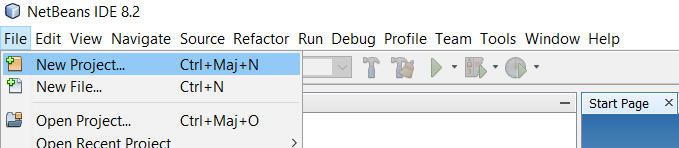
\includegraphics[width=\textwidth]{images/nb_newproject}
			\end{center}
			
			Nommez ce projet \texttt{td-java} et décochez la case \texttt{Create Main Class}.
			
			\begin{center}
				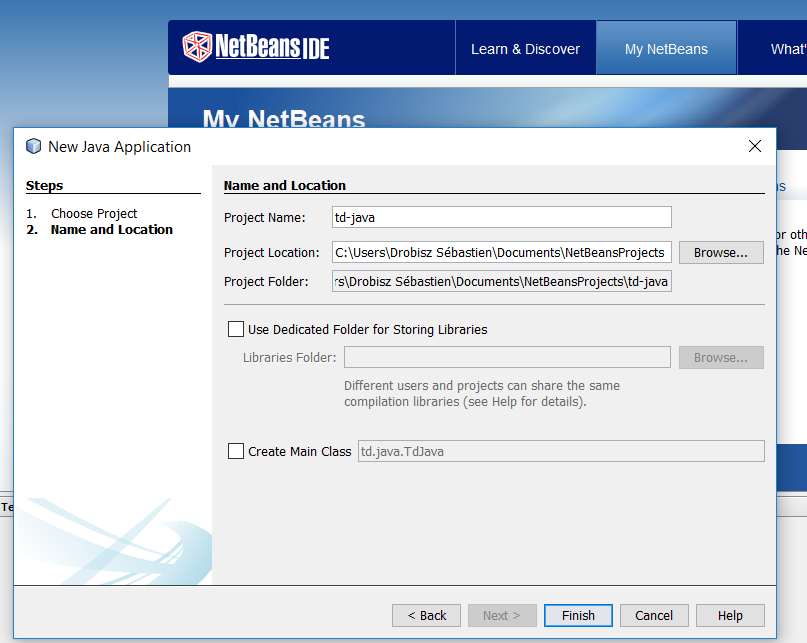
\includegraphics[width=\textwidth]{images/nb_newproject_name}
			\end{center}
			
			Dans NetBeans tout programme doit se trouver au sein d'un projet.
			Le projet contient le code de votre programme mais également les 
			informations annexes comme le langage utilisé (ici Java), 
			la version du langage (ici nous utilisons Java 8), 
			et d'autres informations que vous découvrirez au fur et à mesure.

			% Un répertoire a été ajouté sur votre ordinateur. 	
			% Trouvez le et vérifiez le contenu du dossier contenant les sources de votre projet. 
			% Le dossier sur votre ordinateur s'appelle \texttt{src}. 
			% S'il est vide, c'est normal, vous n'avez pas encore ajouté de source.


		\item Créez un package~: 
		
			faites un clic droit sur le dossier contenant les sources de votre projet, 
			comme illustré dans l'image ci-dessous, et ajoutez un nouveau package Java.
		
			\bigskip
			\begin{center}
				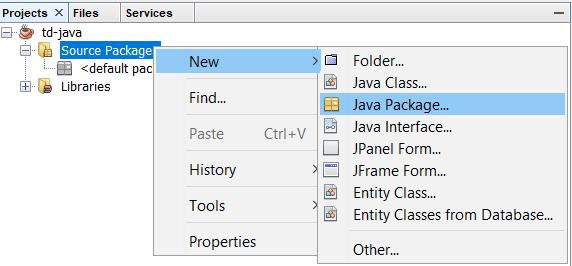
\includegraphics[width=\textwidth]{images/nb_newproject_package}
			\end{center}

			Nommez ce package \texttt{g12345.dev1.td1} où vous remplacez g12345 par votre identifiant~:
			
			\bigskip
			\begin{center}
				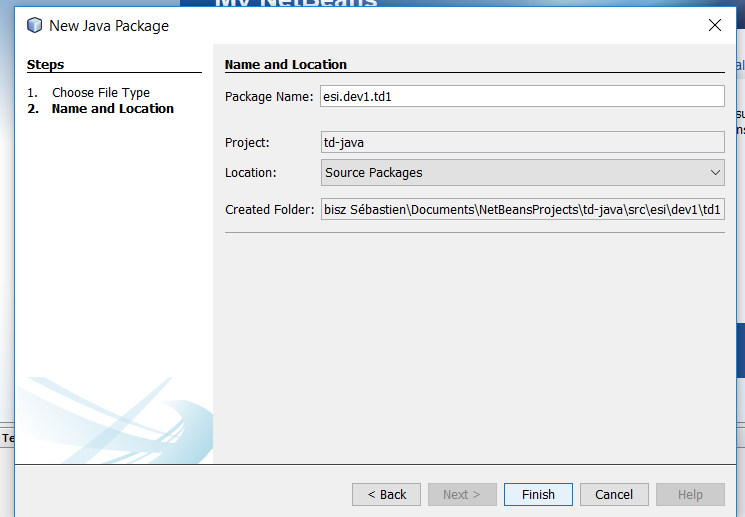
\includegraphics[width=\textwidth]{images/nb_newproject_package2}
			\end{center}
			
			En Java, un package (paquet) permet de regrouper certaines parties de votre code
			et ainsi d'ordonner votre projet.

			Remarquez que ce package a été ajouté dans les sources de votre projet. 
			\bigskip
			\begin{center}
				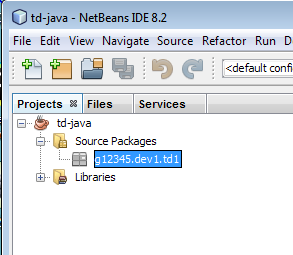
\includegraphics{images/nb_newproject_package3}
			\end{center}
			
			% Dans votre navigateur, vérifiez ce qui a été ajouté dans le dossier contenant vos sources.


		\item Créez une classe~:
		
			comme illustré sur l'image ci-dessous faites un clic droit sur votre package 
			et ajoutez une nouvelle classe\footnote{Pour le moment, 
			on va simplement dire que c'est un fichier dans lequel se trouve du code Java.}. 
			Nommez cette classe {Hello}
			%\footnote{Si vous oubliez la majuscule au H, nous viendrons vous tirer les oreilles !}
		
			\bigskip
			
			\begin{center}
				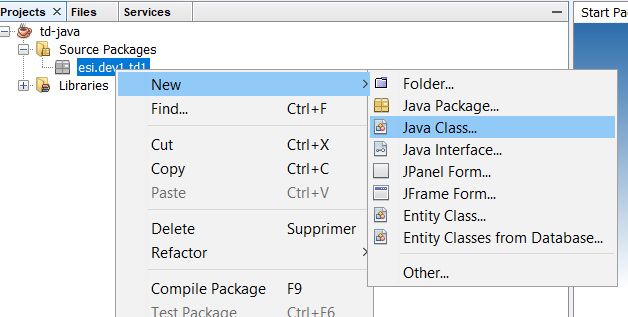
\includegraphics[width=\textwidth]{images/nb_newproject_new_class}
			\end{center}


		\item Ouvrez le fichier \texttt{Hello.java}~:
		
			double-cliquez sur votre classe \texttt{Hello}. 
			Le code se trouvant dans ce fichier apparaît.
			
%			%TODO: enlever le nettoyage ?
%			Si vous voyez le code suivant, 
%			veillez à l'effacer\footnote{Nous n'aimons pas le voir, il ne sert à rien}. 
%			
%			\begin{center}
%				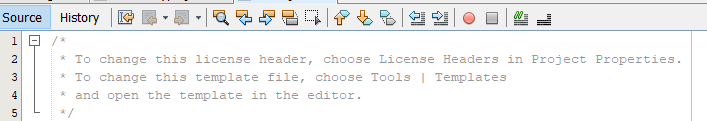
\includegraphics[width=\textwidth]{images/nb_newproject_header}
%			\end{center}
%			
%			Faites la même chose pour le code contenant \texttt{/**...@author...*/}.
			
			Ajoutez le code suivant en respectant bien les 
			minuscules et les majuscules~:
	
			\begin{Code}{java}
				public static void main(String[] args) {
					System.out.println("Hello, World!");
				}
			\end{Code}
			
			Vous devriez obtenir ceci :
			
			\begin{center}
				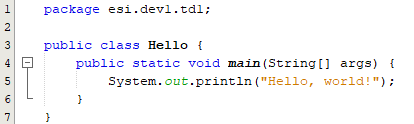
\includegraphics{images/nb_newproject_code}
			\end{center}
			
		\item Lancez le programme en cliquant sur la petite flèche \emph{run} 
			
			
\includegraphics{images/nb_newproject_run}.

		\item Modifiez votre programme pour que celui-ci affiche \texttt{"Hello"} suivi de votre prénom.

	\end{steps}

	\end{Tutoriel}

%===================
\section{Affichage}
%====================	

	Le programme suivant affiche \texttt{Hello!} suivi de \texttt{Bonjour!}.
	\listing{Java}{code/HelloBonjour.java}

	\begin{itemize}
		\item La première ligne indique que la classe se trouve dans le package \texttt{esi.dev1.td1}
		\item La ligne 3 déclare la classe \texttt{HelloBonjour}, remarquez que le nom d'une classe 
			doit correspondre au nom du fichier dans lequel elle se trouve, ici \texttt{HelloBonjour.java}
		\item La ligne 5 déclare la \emph{méthode principale}, \emph{main} en anglais veut dire 'principale'.
			C'est ici que commence votre programme.
		\item En java l'affichage se fait par l'\emph{instruction}: \texttt{System.out.println("Hello!");}
		\item Le texte entre guillemets sera affiché sur la \emph{sortie standard}.
	\end{itemize}


	%Exercices
	\begin{Exercice}{Ligne}
		Dans votre package \texttt{g12345.dev1.td1} créez une classe \texttt{Exercice1}.
		Dans cette classe écrivez un programme  (et donc dans la fonction \texttt{main} de cette classe) 
		qui affiche 10 tirets les uns à la suite des autres:

		\texttt{- - - - - - - - - -}
	\end{Exercice}
	
	\begin{Exercice}{Carré}
		Dans une classe \texttt{Exercice2} (dans votre package \texttt{g12345.dev1.td1}), écrivez un programme qui affiche un carré d'étoiles de 5 de côté:

		\begin{verbatim}
		*****
		*****
		*****
		*****
		*****
		\end{verbatim}
	\end{Exercice}

	\begin{Exercice}{Pyramide}
		Dans une classe \texttt{Exercice3}, écrivez un programme qui affiche une pyramide d'étoiles comme ceci:

		\begin{verbatim}
		   *
		  ***
		 *****
		*******
		\end{verbatim}
	\end{Exercice}



%===================
\section{Expressions}
%====================	

	Le programme suivant affiche la somme de 12345678 et 87654321.
	
	\listing{Java}{code/Expression.java}

	\begin{itemize}
		\item	L'instruction de la ligne 6 affiche le texte entre guillemets~: \texttt{12345678+87654321 = }
	
		\item L'instruction de la ligne 7 affiche le \emph{résultat du calcul} 
			c'est-à-dire la somme de 12345678 et de 87654321~:  \texttt{99999999}
	
		\item Notez que l'\emph{expresssion} \texttt{12345678+87654321} 
			de l'instruction de la ligne 7 ne se trouve \emph{pas} entre guillemets.
	\end{itemize}


	\begin{Exercice}{Petits calculs}
		Dans une classe \texttt{Exercice4}, écrivez un programme qui affiche la valeur des expressions
		suivantes:
		\begin{itemize}
			\item	 \texttt{10 + 32}
			\item	 \texttt{10 - 32}
			\item  \texttt{2 * 21}
			\item  \texttt{234\%57}
			\item  \texttt{((2*2)+(3*3))/25}
		\end{itemize}
	\end{Exercice}
	

%===================
\section{Variables}
%====================	

	Le programme suivant affiche l'aire d'un rectangle de longueur 12 et de largeur 4.
	
	\listing{Java}{code/Variables.java}

	\begin{itemize}
		\item \`A la ligne 6 la variable \texttt{longueur} est \emph{déclarée} 
			avec le type \texttt{int}, elle peut donc 'contenir' des entiers. 
			Sur cette même ligne on lui \emph{assigne} la valeur 12.  

		\item \`A la ligne 7 la variable \texttt{longueur} est \emph{déclarée} avec le type \texttt{int}. 
			Sur cette même ligne on lui \emph{assigne} la valeur 4.
	
		\item \`A la ligne 9 on affiche le résultat de la multiplication de la valeur de la variable \texttt{longueur}, 
			qui vaut 12, et de la valeur de la variable \texttt{largeur}, qui elle vaut 4.  
  	\end{itemize}



	\begin{Exercice}{Petits calculs avec 2 variables} 		
		Dans un classe \texttt{Exercice5} déclarez 2 variables~: 
		\texttt{a}, \texttt{b} et initialisez-les avec les valeurs 51 et 17.
		
		Ensuite affichez sur la sortie standard la valeur de :
		\begin{itemize}
		 	\item a+b
			\item a-b
			\item a*b
			\item a/b
			\item a\%b
			\item a*a+b*b
		\end{itemize} 
	\end{Exercice}

	\begin{Exercice}{Petits calculs avec 3 variables} 
		Dans un classe \texttt{Exercice6} déclarez 3 variables~: 
		\texttt{a}, \texttt{b} et \texttt{c} et initialisez avec les valeurs 2, 3 et 4 respectivement.
		
		Ensuite affichez sur la sortie standard la valeur de :
		\begin{itemize}
		 	\item 4 * a * c
			\item b*b - 4*a*c
		\end{itemize} 
	\end{Exercice}

%===================
\section{Lecture au clavier}
%====================	


	En java la lecture au clavier se fait en 3 étapes.

	\begin{enumerate}
		\item \emph{Importer} le \emph{lecteur} (\texttt{Scanner}) ligne 3 du code ci-dessous.
		\item \emph{Déclarer} et \emph{initialiser} le lecteur:  \texttt{Scanner clavier = new Scanner(System.in);}
		\item La lecture proprement dite: \texttt{int longueur = clavier.nextInt();}
	\end{enumerate}

	\listing{java}{code/AireRectangle.java}


	\begin{Exercice}{Aire d'un carré}
		\'Ecrivez un programme qui demande 
		le côté d'un carré à l'utilisateur et affiche l'aire de ce carré.
	\end{Exercice}

	\begin{Exercice}{Petits calculs avec 2 nombres lus au clavier} 
		\'Ecrivez un programme qui demande 
		deux nombres entiers, \texttt{a} et \texttt{b}, à l'utilisateur et affiche la valeur de :
		\begin{itemize}
		 	\item a+b
			\item a-b
			\item a*b
			\item a/b
			\item a\%b
			\item a*a+b*b
		\end{itemize} 
	\end{Exercice}


\section{Exercices Récapitulatifs}

%	\begin{Exercice}{Triangle}
%		\'Ecrivez un programme qui affiche un triangle d'étoiles comme ceci:
%
%		\begin{verbatim}
%		*
%		**
%		***
%		****
%		***
%		**
%		*
%		\end{verbatim}
%	\end{Exercice}
		
	\begin{Exercice}{Centaines, dizaines, unités} 
		\'Ecrivez un programme qui demande à l'utilisateur 
		un nombre \texttt{nb} compris entre 0 et 1000 et affiche la valeur des expressions suivantes:
		\begin{itemize}
			\item \texttt{nb\%10} - les unités
			\item \texttt{(nb/10)\%10} - les dizaines
			\item \texttt{(nb/100)\%10} - les centaines
		\end{itemize}
		Par exemple, si l'utilisateur entre 362 votre programme affiche
		\begin{verbatim}
		2
		6
		3
		\end{verbatim}
	\end{Exercice}	

	\begin{Exercice}{Miroir} 
		\'Ecrivez un programme qui demande à l'utilisateur 
		un nombre \texttt{nb} compris entre 1000 et 9999 et affiche la valeur miroir:

		Par exemple, si l'utilisateur entre 7362 votre programme affiche 2637.
	\end{Exercice}	

	
	\begin{Exercice}{Secondes en minutes} 
		\'Ecrivez un programme qui demande 
		un nombre de secondes à l'utilisateur
		et qui affiche le nombre de minutes que cela représente.

		Par exemple: 
		si l'utilisateur entre 217 secondes, le programme affiche 3, 
		car 217 secondes correspond à 3 minutes et 37 secondes.
	\end{Exercice}

	\begin{Exercice}{Temps en secondes} 
		\'Ecrivez un programme qui demande 
		une nombre d'heures, un nombre de minutes et un nombre de secondes
		et qui affiche le nombre de secondes totales.
		
		Par exemple: si l'utilisateur entre 2 heures, 10 minutes et 27 secondes, le programme affiche
		7827. En effet 2 heures donnent 7200 secondes, 10 minutes sont 600 secondes 
		auxquelles il faut ajouter les 27 secondes: 7200 + 600 + 27 = 7827. 
	\end{Exercice}

	%TODO: ajoutez quelques exercices



	\newpage
	\begin{Exercice}{Felix}
		\'Ecrivez un programme qui affiche le dessin suivant:

	\begin{verbatim}
	                          :                      :M
	                         XMX                   .HMM>
	                         MMMM.                dMMMM>
	                        'MMMMMX     .....   dMMMMMMX
	                        XMMMMMMMnMMMMMMMMMMMMMMMMMMM
	                       :MMMMMMMMMMMMMMMMMMMMMMMMMMMM>
	                       XMMMMM!"    "MMMMMM"`  `"MMMMM
	                       MMMM#         4MMf        `MMMX
	                      XMMM            MX          'MMM:
	                     'MMM~            '>            MMM
	                     MMMf       .     '>            `MMX
	                    MMMM>     :MMM    '>   :MMM      MMMX
	                   XMMMM      MMMM>   '>   XMMMX     MMMMk
	                  MMMMMM>     MMMM~   'k   MMMMX     MMMMMh
	                 MMMMMMMX     XMMM    XX   ?MMM     XMMMMMMM
	                 MMMMMMMMk     ^`    X 'h    `     :MM##MMM~
	                  ?MM>  ^?M.       .!    %.      .HM"   MM
	                 .?M      '"%+++!".nMMMMn "%++!*" %.. 'M..
	                  `?M>+%L         <MMMMMMMM>       :   XM"
	                    'X   %        XMMMMMMMM>      X   'f
	                      X   `M.      ?MMMMMM~    .HM   :`
	                       %.  `MMMx.          .xHMMM   X
	                  ..    `X  `MMMMMMMMMMMMMMMMMMM  :f
	                :MMMMMMMh:.M. 4MM     "     MM" xMMMMMMMMMMh.
	              :MMMMMMMMMMMMMMM: `%x.......x"`.HMMMMMMMMMMMMMM
	            .MMMMMMMMMMMMMMMMMMMMhx.......xHMMMMMMMMMMMMMMMMM
	    .nHMMMMMMMMMMMMMMMMMMMMMMMMMMMMMMMMMMMM`MMMMMMMMMMMMMMMMX
	  :MMMMMMMMMMMMMMMMMMMMMMMMMMMMMMMMMMMMdMMMMMMMMMMMMMMMMMMMM
	 MMMMMMMMMMMMMMMMMMMM"``""MMMMMMMMMMMM!MMMMMMMMMMMMMMMMMMMM~
	MMMMMMMMMMMMMMMMMMM!     XMMMMMMMMMMMf:HMMMMMMMMMMMMMMMMM!
	M?MMMMMMMMMMMMMMMM`    :MMMMMMMMMMMM!MMMMMMMMMMMMMMMMMMM~
	:MMMMMMMMMMMMMMMMX     MMMMMMMMMMMMXXMMMMMMMMMMMMMMMMM`
	MMMMMMMMMMMMMMMMMX    'MMMMMMMMMMMMM!MMMMMMMMMMMMMMMMX
	MMMMMMMMMMMMMMMMM~    'MMMMMMMMMMMMMM?MMMMMMMMMMMMMMM~
	 #M)MMMMMMMM!MMM       MMMMMMMMMMMMMMMM/MMMMMMMMMMMM~
	   ?MMMMMM"-"2MMMMMx   XMMMMMMMMMMMMMMMMX?**!:MMM"`
	\end{verbatim}
\end{Exercice}




\end{document}
